% Chapter Template

\chapter{Introducción} % Main chapter title
\label{Chapter1}

% Objetivos
% énfasis a la importancia de la temática, su vigencia y  actualidad;
% se  planteará  el  problema  a  investigar,  así  como  el  propósito  o
% finalidad de la investigación.

% TODO: Actualizar con los puntos de este capítulo (X.1, X.2) y una descripcion
%mínima
\chapquote{En este capítulo se se detallarán los motivos por los cuales se ha desarrollado este trabajo. En el apartado \ref{sec:outline} se condensan las intenciones del desarrollo de este trabajo. En el apartado \ref{sec:motivación} se explicará punto por punto qué ha determinado elegir este proyecto. El apartado \ref{sec:proyectos_relacionados} se introduce un estado del arte del las prótesis. El apartado \ref{sec:objetivos} se determina cuál se espera que sea el alcanza de este proyecto. Por último, el apartado \ref{sec:estructura}, resume el contenido del trabajo capítulo por capítulo.}




%%%%%%%%%%%%%%%%%%%%%%%%%%%%%%%%%%%%%%%%%%%%%%%%%%%%%%%%%%%%%%%%
%
%
%        Outline
%
%
%%%%%%%%%%%%%%%%%%%%%%%%%%%%%%%%%%%%%%%%%%%%%%%%%%%%%%%%%%%%%%%%

\section{Síntesis}
\label{sec:outline}


The  EMG  signal  is  a  biomedical  
signal   that   measures   electrical   currents   generated   in   
muscles       during       its       cont
raction       representing       
neuromuscular  activities.


Este trabajo consiste en la creación de un sistema, cuyo objetivo es acercar las
prótesis mioeléctricas al público general. Para ello, los esfuerzos se han
centrado en la creación de un modelo protésico mediante impresión 3D, el montaje del
mismo y sus componentes electrónicos, investigación sobre las distintas formas de captar
las señales electromiográficas (estas señales miden las corrientes eléctricas generadas en los músculos durante su contracción \cite{emg}) y la aplicación de algoritmos de aprendizaje artificial para la
clasificación de estas señales. A estos últimos apartados dedicaremos la mayor parte del
esfuerzo de este trabajo, con su posterior evaluación y comparación de los resultados de
cada algoritmo, a fin de constatar si es viable la creación de un sistema que sea robusto
para ser usado \textit{a posteriori}, como base de la creación de una prótesis de
miembro superior mioeléctrica, inteligente y de bajo coste.




%%%%%%%%%%%%%%%%%%%%%%%%%%%%%%%%%%%%%%%%%%%%%%%%%%%%%%%%%%%%%%%%
%
%
%        Motivación
%
%
%%%%%%%%%%%%%%%%%%%%%%%%%%%%%%%%%%%%%%%%%%%%%%%%%%%%%%%%%%%%%%%%

\section{Motivación}
\label{sec:motivación}

Este trabajo surge de la necesidad de dar forma a todos los conocimientos adquiridos
a lo largo de la carrera, así como de aunar y profundizar
en las pasiones descubiertas estos años. Así pues, este proyecto ha sido fuertemente influenciado por:

\begin{itemize}
  \item Parte de inteligencia artificial.
    \begin{itemize}
      \item 34024 - Sistemas Inteligentes.
      \item 34031 - Razonamiento Automático.
      \item 34032 - Desafíos de programación.
      \item 34034 - Procesamiento de Lenguajes.
      \item 34030 - Visión Artificial y Robótica.
    \end{itemize}


  \item Parte de microcontroladores y robótica.
    \begin{itemize}
      \item 34036 - Tecnología y Arquitectura Robótica.
      \item 34049 - Sistemas Embebidos.
      \item 34050 - Sistemas Industriales.
    \end{itemize}

  \item Desarrollo personal.
    \begin{itemize}
      \item Curso CECLEC Taller impresoras 3D REPRAP, \textit{Universidad de
        Alicante}.
      \item Introduction to Computational Thinking and Data Science,
        \textit{Massachusetts Institute of Technology through edX}.
    \end{itemize}
\end{itemize}


Otra necesidad ha sido poder desarrollar y trabajar sobre un prototipo real,
teniendo en mente poder aplicar todos los conocimientos mencionados
anteriormente
sobre éste. Por tanto, la impresión 3D ha tenido un papel fundamental, debido a que el uso
de cualquier otra tecnología para este fin habría sido ineficiente debido a su
alto coste.



\subsection{Motivación social}
\label{sub:Motivación-social}

Según la Asociación Nacional de Amputados (Adampi), se calcula que unas 50.000
personas en España llevan prótesis \cite{mundo-10-barbaridad}, sin contar con las que no han podido
costeárselas o quienes las adquieren por el sector privado. Además, un 10\% del
total son niños en edad de crecimiento \cite{abc-olvidados}.

Una amputación no es solo un problema fisiológico, sino que repercute en la
persona a nivel psicológico, social y económico, por lo que no basta solo con
facilitar ayudas para adquirir una prótesis y esperar que la persona tenga
suficiente dinero para pagar el porcentaje restante o que sea ella quien se
tenga que adaptar a la prótesis y no viceversa.

En esta línea se ha hecho el estudio El impacto emocional de la Ayuda Técnica
(2013), que destaca el ``papel integrador'' de las prótesis para este colectivo
y recoge sus principales demandas, que son:

\begin{itemize}
  \item \textbf{Una prótesis adecuada a las necesidades} : Una prótesis para un
	niño o niña en edad de crecimiento va a necesitar ser sustituida cada poco tiempo
	además de resistente, ya que son susceptibles de romperse cuando éstos/as
	juegan; una persona joven va a necesitar una prótesis funcional y que le
	facilite la integración laboral, y una persona mayor quizá no va a requerir
	una prótesis tan resistente pero sí que se adapte a ella. También habrá que
	valorar el estilo de vida de cada persona para poder ofrecer una prótesis
	adecuada a sus necesidades.

  \item \textbf{Cambiar la visión actual sobre el gasto social}: El gasto social
  	es realmente una inversión, tanto para mejorar el bienestar y la calidad de
	vida de las personas, como para ahorrar futuros gastos derivados de un
	recurso inadecuado. Además, favorece la integración laboral, lo que supone
	una inversión para el Estado y la recuperación del dinero destinado al gasto
	social.

  \item \textbf{Facilitar los procesos de adquisición y/o cambio}: Al tratarse
  	de un proceso parcialmente administrativo, puede resultar lento y complejo.
	Esto dificulta la realización de las actividades diarias así como la
	normalización de la situación de la persona.

\end{itemize}

En España, distintas asociaciones han puesto de manifiesto su disconformidad
sobre el actual sistema de subvenciones que estipula el Real Decreto 1506/2012
aprobado por el Ministerio de Sanidad \cite{boe}. Así, a día de hoy, muchas familias tienen
que pagar el 10\% de las prótesis, lo que puede suponer 3000\euro~en algunos casos,
sin tener en cuenta que, como ya hemos comentado, se deben renovar cada pocos
años en el caso de niños y niñas. Por otro lado, las prótesis no han sufrido un
proceso de evaluación y mejora, por lo que han quedado obsoletas o
desactualizadas; sin embargo, los precios actuales son los estipulados por este
decreto en el año 2012, que son elevados para el nivel de calidad de vida que
aportan.


En cuanto al aspecto psicológico, es sabido que las personas con amputaciones
tienen dificultades para la participación e integración social. Estas personas
se pueden encontrar con falta de autonomía para realizar tareas básicas,
frustración e incluso aislamiento social. El hecho de que puedan contar con una
prótesis de calidad y adaptada a su condición supone un impacto emocional
positivo que facilita que la persona vuelva a tener confianza en sí misma y
aumente su bienestar social y emocional y su calidad de vida.

Todo esto es lo que ha motivado la realización de este proyecto que, en
definitiva, pretende solventar estos problemas mediante el desarrollo de una
prótesis mioeléctrica impresa en 3D que ofrece un modelo funcional y
actualizado, para el que se necesita un bajo coste de producción, lo que
repercutirá en el precio final de mercado, que será menor que el actual y por
tanto podrá facilitar su adquisición a más personas. Asimismo, se han utilizado
tecnologías libres para que las personas interesadas puedan aportar ideas y/o mejoras a este proyecto.




%%%%%%%%%%%%%%%%%%%%%%%%%%%%%%%%%%%%%%%%%%%%%%%%%%%%%%%%%%%%%%%%
%
%
%        Proyectos relacionados
%
%
%%%%%%%%%%%%%%%%%%%%%%%%%%%%%%%%%%%%%%%%%%%%%%%%%%%%%%%%%%%%%%%%

\section{Proyectos relacionados}
\label{sec:proyectos_relacionados}

Como veremos a continuación, existen diversos proyectos, que se han desarrollado
en los últimos años en el ámbito de las prótesis. Esto es debido, en gran parte,
al denominado movimiento \textit{maker} y al cada vez más fácil acceso de las
impresoras 3D por parte del público general.

En las siguientes subsecciones, se hará un repaso de los proyectos que se
están desarrollando actualmente, con el fin de contextualizar las diversas
técnicas empleadas en este trabajo en el sector de las prótesis de miembro
superior.


%-----------------------------------
%	SUBSECTION 1
%-----------------------------------
\subsection{Automail}
\label{sub:automail}

Proyecto hecho público recientemente \cite{enable-myo} (25 marzo de 2016)
que comparte algunos componentes con los de este trabajo. Consiste en una
aplicación python diseñada para ser cargada en una Raspberry Pi \cite{raspberry-pi}
y que actúa de puente entre la Myo Armband~\ref{subs:myo} y un Arduino~\ref{subs:arduino}.

El funcionamiento \cite{automail} consiste en sincronizar la Myo Armband con una Raspberry Pi y
ésta a un Arduino, que se encargará de girar una base conectada a un motor
servo, el cual hará girar la prótesis sobre su eje z. El giro hacia la izquierda
o derecha depende de si la mano está abatida haca dentro o fuera
respectivamente.

Por otra parte, es capaz de mandar una señal a la prótesis si se cierra el puño
para agarrar objetos o de soltarlo si se separan los dedos.

\begin{figure}[h]
    \centering
    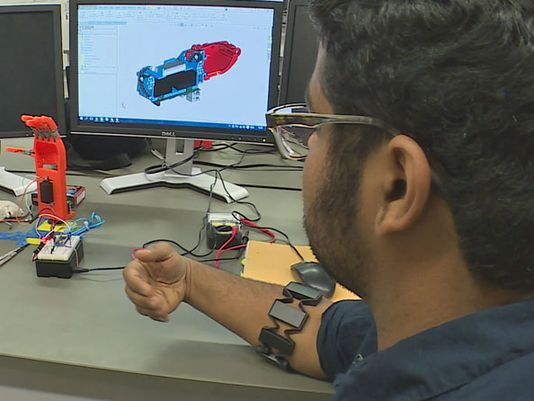
\includegraphics[width=0.7\textwidth]{Chapter1/automail}


\caption{Muestra del proyecto Automail en acción. Figura extraida de legacy.king5.com}
%http://legacy.king5.com/story/tech/science/2015/10/13/students-develop-technology-to-make-prosthetics-more-affordable/73901962/
\label{fig:automail}
\end{figure}


Este proyecto destaca por la correcta integración de los distintos
componentes (Myo, Raspberry Pi y Arduino). No obstante, al no estar
especificado,
se entiende que el proceso de reconocimiento de poses es el que viene
implementado por defecto en la Myo, el cual, al actuar como caja negra, es
imposible saber cómo funciona y, mucho menos, poder modificarlo para nuestras
necesidades.



%-----------------------------------
%	Inmoov
%-----------------------------------
\subsection{Inmoov}
\label{subs:inmoov}

Inmoov nace como proyecto personal de Gael Langevin, con el objetivo de crear
un robot humanodide hecho con tecnología de impresión 3D, completamente
funcional y libre \cite{langevin2014inmoov}. La relación con este proyecto surge
del uso que le ha dado la comunidad, ya que, al ser libre, se ha decidido utilizar
el brazo (Figura~\ref{fig:inmoov}) como prótesis.

\begin{figure}[htp]
  \centering
    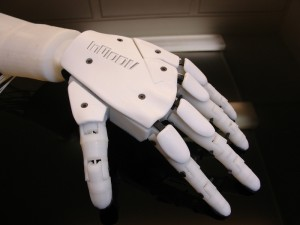
\includegraphics[width=0.8\textwidth]{Chapter1/inmoov}
  \caption{Mano y parte del brazo del proyecto Inmoov.}
\label{fig:inmoov}
\end{figure}

Inmoov destaca por su documentación sobre la construcción de la mano, que lo ha hecho
relativamente popular. Por contrapartida, el proyecto tiene un caracter
más conceptual que %TODO: rellenar esta parte y revisar todo este párrafo,
siendo habitual verlo como parte de exposiciones en museos y en algunas ferias
tecnológicas. Esto, aunque pueda parecer que no es una gran inconveniencia, en
la práctica se está viendo cómo nuevas versiones de la mano y el antebrazo están
dejando de ser 100\% libres. Por parte de la comunidad se ve bastante
actividad, pero no documentada, por lo que son simples bancos de pruebas sin desarrollar
aplicaciones serias.



%-----------------------------------
%	Open Bionics
%-----------------------------------
\subsection{Open Bionics}
\label{sub:open-bionic}

Conocida anteriormente como Open hand project, es una empresa incubada en el
Laboratorio de Robótica de Bristol que tiene como objetivo la creación de
prótesis de mano impresas en 3D y de bajo coste \cite{remenyi2015innovation}.
Este proyecto ha participado en distintas competiciones, donde destaca
el 2º puesto en Make it wereable de Intel 2014 y el 1º puesto en Innovación en
ingeniería
de los premios James Dyson 2015. Estos premios, entre otros, han permitido
que el proyecto siga desarrollándose. Actualmente, están trabajando
con la prótesis Ada (Figura~\ref{fig:ada}), así como su propio
microcontrolador PCB, el Almond PCB.
% TODO: incluir acrónimo PCB



\begin{figure}[htp]
  \centering
    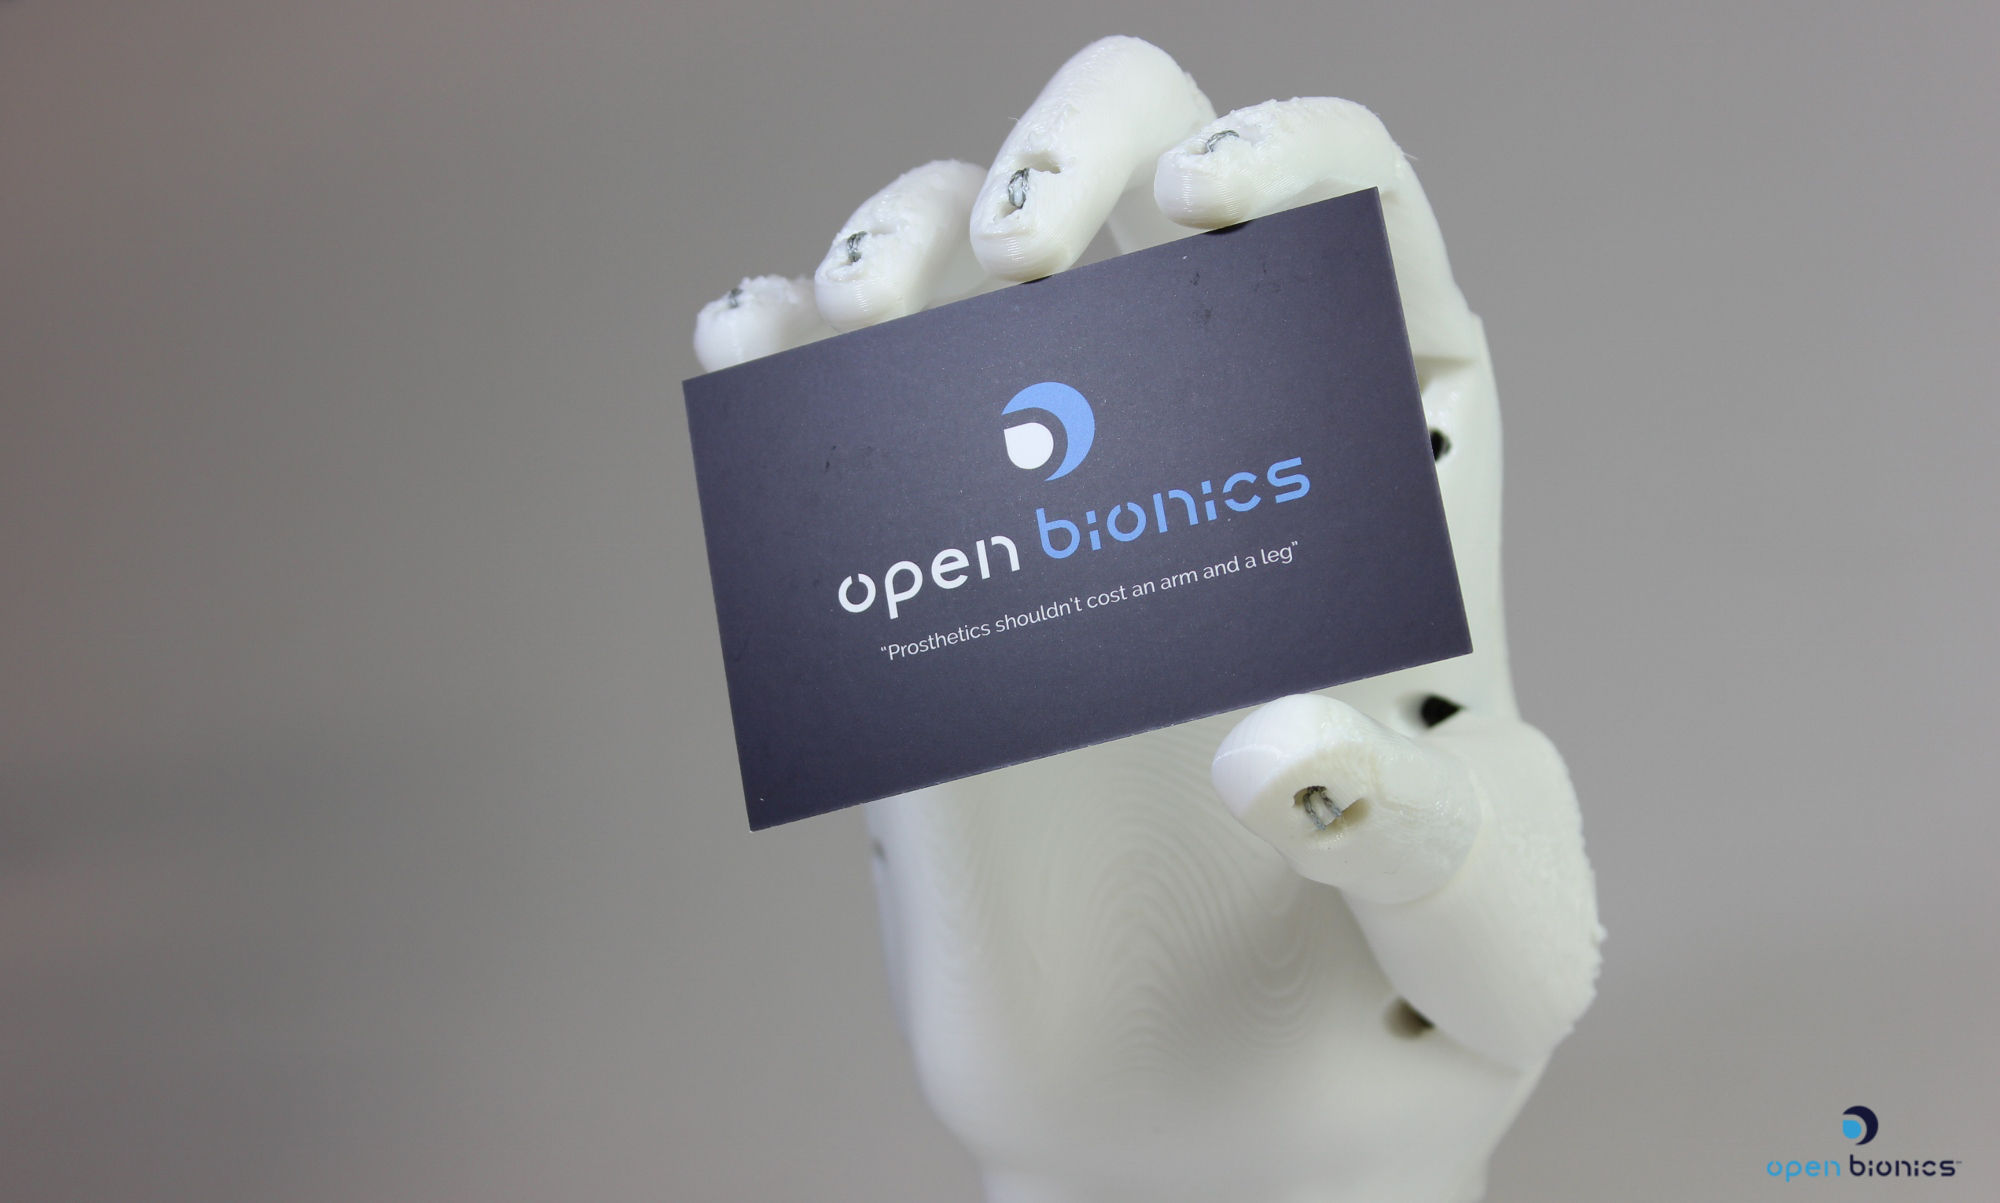
\includegraphics[width=0.8\textwidth]{Chapter1/ada}
  \caption{Ada, el último modelo de prótesis desarrollado por Open Bionics.}
\label{fig:ada}
\end{figure}


El modelo Dextrus, anterior a Ada, fue desarrollado en los inicios de esta
empresa
como parte del proyecto Open hand project. En la figura~\ref{fig:dextrus} se
muestra
una mano impresa basada en los modelos 3D Dextrus.


\begin{figure}[htp]
  \centering
    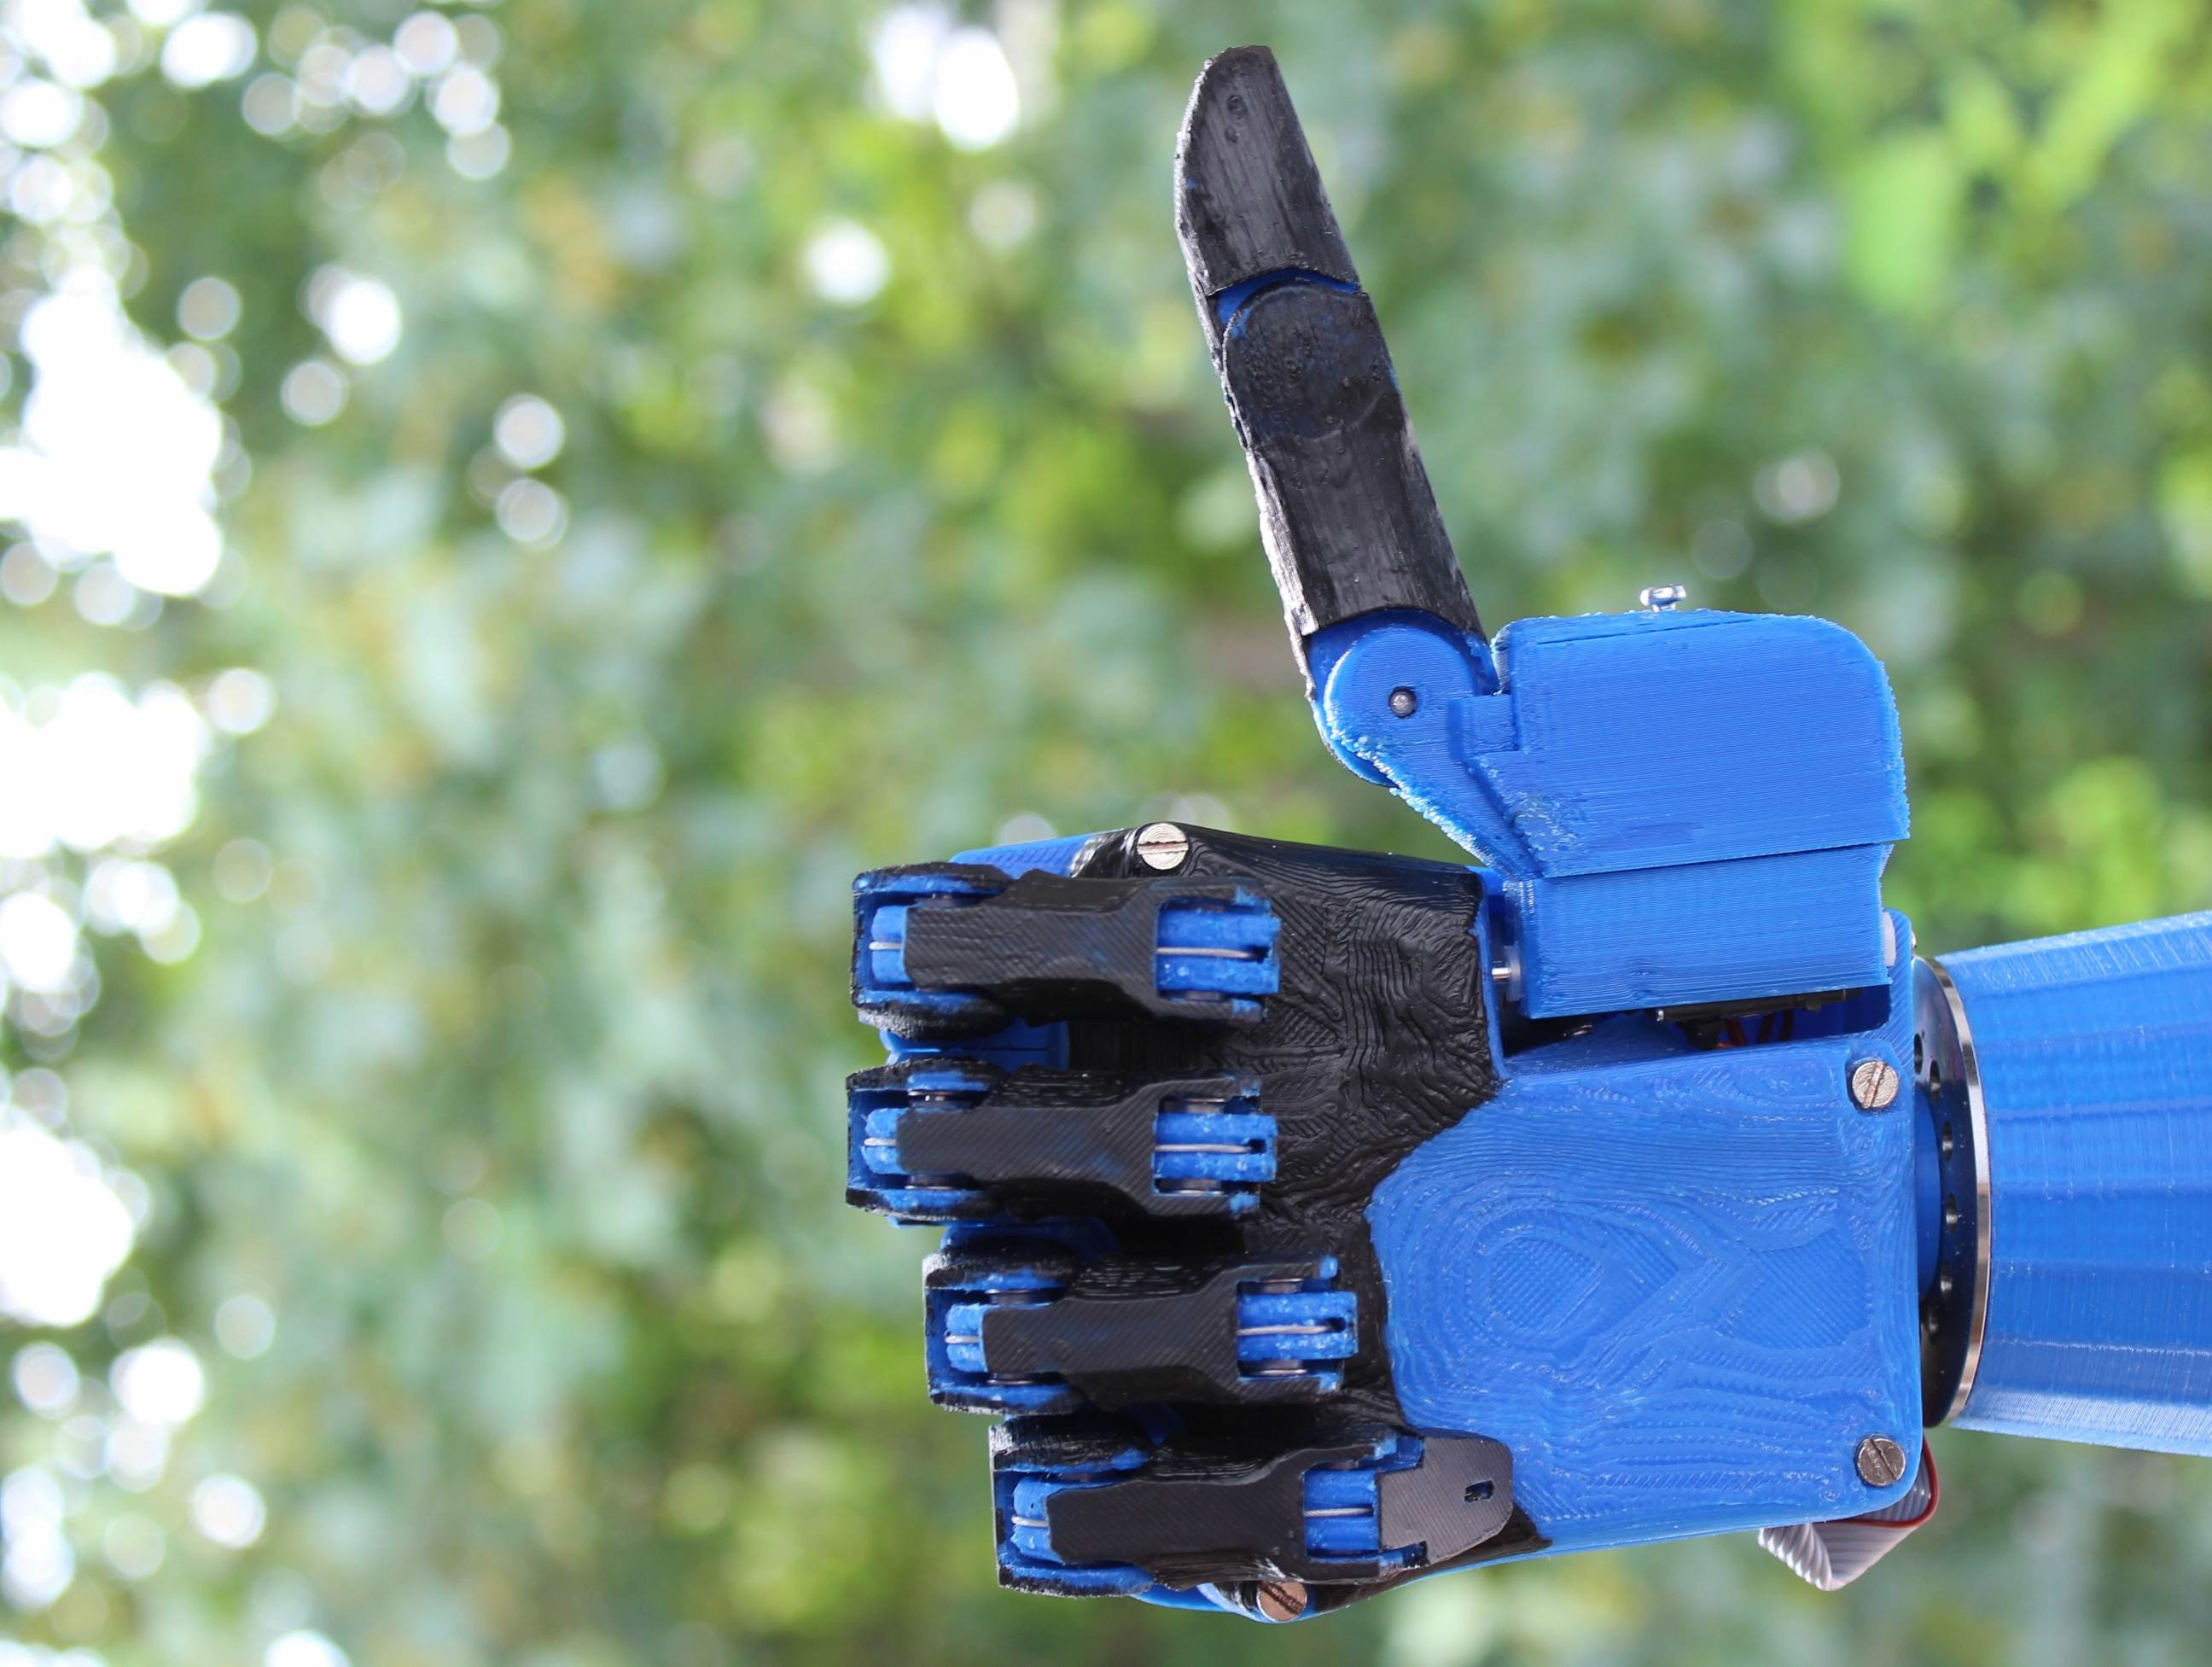
\includegraphics[width=0.65\textwidth]{Chapter1/dextrus}
  \caption{Prótesis Dextrus con el pulgar levantado.}
\label{fig:dextrus}
\end{figure}

%TODO: terminar apartado de OB con la conclusión


\subsection{Bebionic}
\label{sub:bebionic}

La prótesis mioeléctrica de mano Bebionic está diseñada por la empresa
RSLSteeper.
Esta prótesis viene preprogramada con múltiples posiciones de agarre y es
controlada
por la contracción de los músculos, como la mayoría de prótesis mioeléctricas
\cite{medynski2011bebionic}.

Esta prótesis, como se puede apreciar en al figura~\ref{fig:bebionic}, se
caracteriza por usar los materiales y técnicas más avanzadas actualmente. Es capaz de
realizar 14 posiciones o patrones de agarre distintos, además de poder usar el
pulgar de forma abatible (que ha de accionarse manualmente). La electrónica se
encarga de realizar una monitorización de cada motor (uno por cada dedo) para
reproducir correctamente los patrones y maximizar la precisión de cada
movimiento \cite{medynski2011bebionic}.


\begin{figure}[htp]
  \centering
    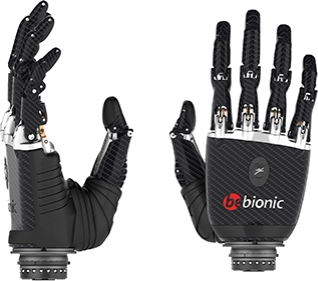
\includegraphics[width=0.6\textwidth]{Chapter1/bebionic}
  \caption{Perfil y reverso de Bebionic}
\label{fig:bebionic}
\end{figure}

% TODO: añadir RF a acrónimos (radiofrequencia)

El software que acompaña esta prótesis es Bebalance desarrollado por la propia
RSLSteeper. Toda la información es transmitida desde y hacia este sistema
mediante un emisor y receptor RF incorporado en la prótesis
\cite{waryck2011comparison}.
Bebalance permite, entre otras cosas, la configuración de la presión que puede
ejercer o la velocidad de los motores. Es posible también realizar un
seguimiento visual de los sensores mediante monitores de análisis en tiempo
real, permitiendo al usuario practicar mediante un \textit{feedback} real de
los sensores \cite{medynski2011bebionic}.

RSLSteeper autodenomina esta prótesis como ``La prótesis de mano más avanzada
del mundo'' \cite{bebionicWeb}. Por ello, y por su precio, que oscila entre
los 25.000\$ y los 35.000\$ \cite{bebionicPrice}, se ha tomado como cota
máxima
de lo que una prótesis, actualmente, puede hacer y qué limitaciones tiene.



\subsection{Propósitos}
\label{sub:propósitos}

Después de entender la motivación de este TFG y conocer el estado de desarrollo de los proyectos
relacionados que se están llevando a cabo hasta el momento, este trabajo pretende lograr:

\begin{itemize}
  \item Reducción del coste final de una prótesis de mano mioeléctrica.
  \item Crear un sistema de detección de patrones robusto.
  \item Los movimientos de la prótesis deben adecuarse de forma realista a las
  acciones hechas por el usuario.
  \item Facilitar el uso y configuración de la prótesis a usuarios no expertos.
  %TODO revisar penúltimo punto
\end{itemize}


\section{Objetivos}
\label{sec:objetivos}


El objetivo final es que una prótesis impresa en 3D sea capaz de reproducir
el movimiento natural de una mano real. Estos movimientos han de ser la respuesta a los impulsos
eléctricos del músculo del usuario, que son captados mediante un dispositivo
con sensores de señales EMG (siglas para electromiografía).

El proceso de identificación de qué movimiento debe realizar la prótesis será
implementado usando técnicas de inteligencia artificial, más concretamente,
algoritmos de clasificación.

% TODO: indicar la sección o capítulo
El proceso de aprendizaje, como veremos más adelante en \ref{sec:clasificación-señales-emg},
requiere una gran cantidad de colección de datos de todos los movimientos que se quieren
reproducir, por lo que, teniendo en cuenta que cada usuario será distinto, se facilitará una
forma lo más sencilla posible de obtener la cantidad de datos necesaria que
se precise para el correcto funcionamiento del proceso de clasificación.

Para asegurar que el sistema final sea robusto, se especificarán distintos
movimientos y se recopilarán los conjuntos de datos necesarios para aplicar distintos
algoritmos, así como distintas técnicas para decidir de forma objetiva qué algoritmo
funciona mejor con el tipo de dato que proporciona el dispositivo EMG y que será empleado
en el producto final.

Por último, aunque todo el proceso de desarrollo del sistema se haga en forma
de prototipo, se deberá realizar un análisis de la viabilidad de la exportación
del trabajo a un entorno real, es decir, estimar la vida útil de la prótesis con
las baterías actuales disponibles o comprobar si el precio de los componentes
necesarios para un entorno real no superan los límites para que la prótesis siga
considerándose de bajo coste.


\section{Estructura}
\label{sec:estructura}

Este TFG se ha estructurado de la siguiente forma:

\begin{itemize}
	\item Capítulo \ref{Chapter1}: se resume el proyecto y los motivos por el que se ha desarrollado. Se incluye también, un estado del arte sobre las prótesis y proyectos más destacables sobre las mismas.
	\item Capítulo \ref{Chapter2}: aúna las herramientas utilizadas para el desarrollo de la prótesis y de su sistema de control.
	\item Capítulo \ref{Chapter3}: introducción a los algoritmos de aprendizaje automáticos, con especial hincapié en  los modelos de redes neuronales artificiales.
	\item Capítulo \ref{Chapter4}: descripción de los métodos desarrollados para la obtención del conjunto de datos que será utilizado a su vez, por el modelo de aprendizaje para clasificar las señales EMG.
	\item Capítulo \ref{Chapter5}: conclusiones sobre los resultados obtenidos y propuestas para continuar y mejorar el trabajo realizado.
\end{itemize}
